\documentclass[tikz,border=6pt]{standalone}
\usepackage{xcolor}

\definecolor{blockblue}{HTML}{4A90D9}

\begin{document}
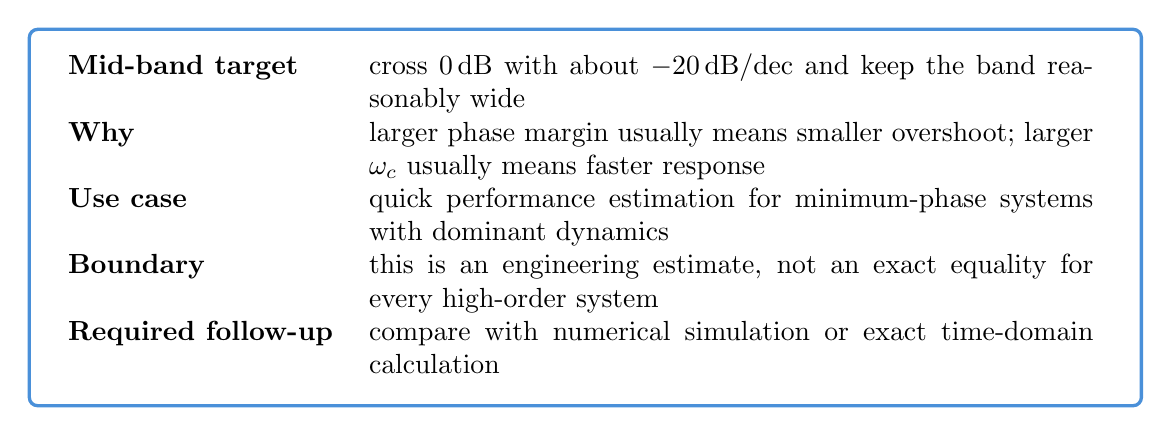
\begin{tikzpicture}[line width=1.2pt]
  \node[
    draw=blockblue,
    rounded corners=3pt,
    inner sep=8pt,
    align=left
  ] at (0,0) {
    \begin{tabular}{p{3.4cm}p{9.2cm}}
      \textbf{Mid-band target} & cross $0\,\mathrm{dB}$ with about $-20\,\mathrm{dB/dec}$ and keep the band reasonably wide \\
      \textbf{Why} & larger phase margin usually means smaller overshoot; larger $\omega_c$ usually means faster response \\
      \textbf{Use case} & quick performance estimation for minimum-phase systems with dominant dynamics \\
      \textbf{Boundary} & this is an engineering estimate, not an exact equality for every high-order system \\
      \textbf{Required follow-up} & compare with numerical simulation or exact time-domain calculation \\
    \end{tabular}
  };
\end{tikzpicture}
\end{document}
